

\documentclass[10pt,twocolumn,letterpaper]{article}

\usepackage{cvpr}
\usepackage{times}
\usepackage{epsfig}
\usepackage{graphicx}
\usepackage{amsmath}
\usepackage{amssymb}
\usepackage{algorithm}

\usepackage{algpseudocode}

\usepackage{url}

% Include other packages here, before hyperref.

% If you comment hyperref and then uncomment it, you should delete
% egpaper.aux before re-running latex.  (Or just hit 'q' on the first latex
% run, let it finish, and you should be clear).
%\usepackage[pagebackref=true,breaklinks=true,letterpaper=true,colorlinks,bookmarks=false]{hyperref}

\cvprfinalcopy % *** Uncomment this line for the final submission

\def\cvprPaperID{****} % *** Enter the CVPR Paper ID here
\def\httilde{\mbox{\tt\raisebox{-.5ex}{\symbol{126}}}}

% Pages are numbered in submission mode, and unnumbered in camera-ready
\ifcvprfinal\pagestyle{empty}\fi
\begin{document}

%%%%%%%%% TITLE
\title{Comparative analysis between sequencial and parallel version of the K-means algorithm in C++ }

\author{Francesco Bongini\\
\tt\small bongini.francesco@gmail.com}
% For a paper whose authors are all at the same institution,
% omit the following lines up until the closing ``}''.
% Additional authors and addresses can be added with ``\and'',
% just like the second author.
% To save space, use either the email address or home page, not both

\maketitle
\thispagestyle{empty}

%%%%%%%%% ABSTRACT
\begin{abstract}
For physical limitations, in the recent decades computers have increased the number of cores rather than increasing the speed of each one.
To get the best beneficts of the computational power, we need to build new versions of existing algorithms.
This paper presents the results of a comperative analysis between sequencial
and parallel version of the K-means clustering. The parallel code is implemented using OpenMP in C++.
My results indicate that the parallel implementation has benefits regarding its speed and the amount of data processed in the same quantity of time. 
\end{abstract}


\section{Introduction}
K-means is a simple unsupervised learning algorithm that is used to solve clustering problems. 
Definited the parameter \emph{K} i.e. the numer of clusters, the algorithm chooses randomly \emph{K} points (called centroids).
Each point of the dataset is assigned to the cluster with the closest centroid.
After all points are assigned, the positions of the \emph{k} centroids are recalculated with the mean of the cluster.
The algorithm repeates the recalculates until the centroids don't change more.
Here the pseudocode of the K-means clustering:
\begin{algorithm}

\label{Kmeans}

\caption{Kmeans}


1: Select K points as the initial centroids.\\
2: repeat\\
3: Form K clusters by assigning all points to the closest centroids.\\
4: Recompute the centroid of each cluster with the mean of the points in each cluster.\\
5: Until the centroids don't change.
\end{algorithm}
\\
\begin{figure}[H]
\centering
\includegraphics[width=8.5cm]{{"C:/Users/Francesco/Desktop/unifi/Magistrale/Parallel Computing/Progetto/Immagini/esempioKmeans"}.png}
\caption{Kmeans algorithm in different iterations}\label{example}
\end{figure}
Given two points $p$ and $q$ in $n$ dimensions, their euclidean distance is defined as: $$d(p,q)=\sqrt{\sum_{i=1}^{n}(p_i-q_i)^2}$$ 

\section{Plotting clusters}
After have calculated the clusters with Kmeans algorithm, we plot them. Python provides interesting libraries to plot our clusters in 3D.\\
The dataset is a mixture of 3 dimensions points from Gaussian distributions with mean 0, 3 and 6 and standard deviation equal to 0.2 for each one. 
Given the standard deviation very small, the algorithm converges in barely 4 iterations. Here the plots in 2 and 3 dimensions:\\ \\
\begin{figure}[H]
\centering
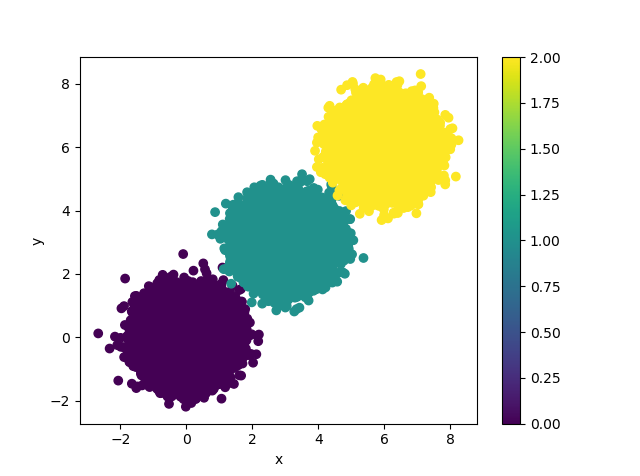
\includegraphics[width=6.5cm]{{"C:/Users/Francesco/Desktop/unifi/Magistrale/Parallel Computing/Progetto/Immagini/cluster2D}.png}
\caption{Plot clusters in 2 dimensions}\label{2D}
\end{figure}
\begin{figure}[H]
\centering
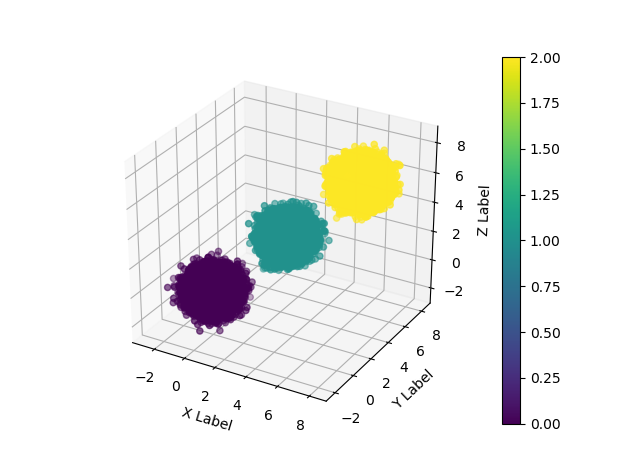
\includegraphics[width=7.7cm]{{"C:/Users/Francesco/Desktop/unifi/Magistrale/Parallel Computing/Progetto/Immagini/cluster3D}.png}
\caption{Plot clusters in 3 dimensions}\label{3D}
\end{figure}




\section{Sequential version}
Sequential version of the Kmeans algorithm consists to calculate and update the new centroids until they differ from the old centroids less than the $\epsilon$ value. 
Here is the pseudocode of the sequential version:
\begin{algorithm}
\label{sequenziale}
\caption{Sequential version}
\begin{algorithmic}
	\While{centroids change}
    		\For{each point}
			\State point.setCluster()
		\EndFor
    		\State upgradeCentroids();
   	 \EndWhile
\end{algorithmic}
\end{algorithm} 
\\
The choice of the $\epsilon$ value may affect the speed and the precision of the algorithm. The points are definited as PointND object. It consists in vector of floats i.e. the coordinates and the attribute Cluster. Cluster is an integer-type that indicates the class to which each point corresponds. During each iteration of the kmeans the points don't change, but may occur to the Cluster. An other important data structure is the vector of PointND, used to define the list of centroids.
Each point of the dataset is visited sequentially to calculate the distance from the $K$ centroids.

\section{Parallel version}
OpenMP  is  a  standard  Application  Programming 
Interface of C, C++ and FORTRAN for a shared memory 
parallel programming. It allows to parallel the exacution of Kmeans in a very simple way.
In fact, after definited the number of $threads$, the command \emph{\#pragma omp parallel for} allows to each $thread$ to compute an 
indipendent part of the data. This is possible because the iterates of the loop are indipendent of each other and the number of iterates is known in advance. 
Given that the steps are the same for each data point, static schedule is assigned by default.
Here is the pseudocode of the parallel version:
\begin{algorithm}
\label{parallelo}
\caption{Parallel version}
\begin{algorithmic}
	\While{centroids change}
		\State \#pragma omp parallel for
    		\For{each point}
			\State point.setCluster()
		\EndFor
    		\State upgradeCentroids();
   	 \EndWhile
\end{algorithmic}
\end{algorithm}
\\Note that "upgradeCentroids()" isn't parallelized. If we parallelize that with \emph{Pragma OpenMP}, different data points might be added to the sum of them to calculate the centroid
 at the same time, leading to Write-After-Write (WAW) hazard. It happens when different threads save their results to the same variable causing the loss of results of the previous threads.


\section{Speedup}
Speedup is an index that measures the relative performance of two systems processing the same problem.
It is defined as: $$S_p=t_s/t_p$$ where P is the number of processors, $t_s$ is the completion time of the sequential 
algorithm and $t_p$ is the completion time of the parallel algorithm. Here is some Speedup types:
\begin{figure}[H]
\centering
\includegraphics[width=5.5cm]{{"C:/Users/Francesco/Desktop/unifi/Magistrale/Parallel Computing/Progetto/Immagini/types"}.png}
\caption{Speedup types}\label{types}
\end{figure}
Types:\\
1. Linear speedup\\
2. Sub-linear speedup\\
3. Speedup with an optimal number of processors\\
4. No speedup\\
5. Super-linear Speedup\\
\\
In order to analyze the speedup for this problem, different datasets are considerated.
The first example shows the results from the hardware of my laptop. 
In the other examples I used an istance from Amazon AWS.

\subsection{500k points}
\textbf{Dataset}: 500k points in 3 dimensions from Gaussian distribution with mean 0 and standard deviation 1. \\
\textbf{Parameters}: $\epsilon$=0.001 and $K$=3. \\
\textbf{Processor}: Intel(R) Core(TM) i5-6200U CPU @ 2.30GHz, 2401 Mhz, 2 Core(s), 4 Logical Processor(s). \\
\textbf{number iterations}: 121 \\
\textbf{Results}\\
1 thread:{ } \quad186.833 seconds\\
2 threads: \quad131.318 seconds\\
3 threads: \quad128.658 seconds\\
4 threads: \quad109.824 seconds\\
5 threads: \quad113.157 seconds\\
6 threads: \quad111.582 seconds\\
7 threads: \quad112.294 seconds\\
Increasing the number of threads overhead increases, so we need to find the optimal number of threads.

\subsection{2M points}
\textbf{Dataset}: 2 millions points in 4 dimensions from Gaussian distributions with mean 1 and standard deviation 1. \\
\textbf{Parameters}: $\epsilon$=0.001 and $K$=3. \\
\textbf{Processor}: t2.2xlarge Linux/UNIX Amazon Ec2 Spot Instance with 8 vCPUs. \\
\textbf{number iterations}: 229\\
\textbf{Results}:\\
1 thread:{ } \quad 929.932 seconds\\
2 threads: \quad554.635 seconds\\
3 threads: \quad434.368 seconds\\
4 threads: \quad375.278 seconds\\
5 threads: \quad340.358 seconds\\
6 threads: \quad317.651 seconds\\
7 threads: \quad301.631 seconds\\
8 threads: \quad295.699 seconds\\
9 threads: \quad317.819 seconds\\
10 threads:\quad307.321 seconds\\
\begin{figure}[H]
\centering
\includegraphics[width=7.5cm]{{"C:/Users/Francesco/Desktop/unifi/Magistrale/Parallel Computing/Progetto/Immagini/bar2M"}.png}
\caption{Bar chart}\label{bar2M}
\end{figure}
\begin{figure}[H]
\centering
\includegraphics[width=7.5cm]{{"C:/Users/Francesco/Desktop/unifi/Magistrale/Parallel Computing/Progetto/Immagini/speedup2M"}.png}
\caption{Speedup OpenMP}\label{speedup2M}
\end{figure}

\section{Further parallelization}
A further parallelization of the problem is possible. In fact, after calculating the distance between points and centroids, it's possible to
parallelize the external loop of the calculation of the new centroids. In this way, each thread calculate the new centroid of a different cluster.
For istance, thread 0 computes the cluster 0, thread 1 computes the cluster 1 etc.. . It is important therefore that $K$ is big enough, to use 
all cores availables. Given that the steps are the same for each cluster, there are slight differences between static and dynamic schedule.
Static schedule is assigned by default.\\
Here is the pseudocode of the new parallel version:
\begin{algorithm}
\label{newparallelo}
\caption{Parallel version}
\begin{algorithmic}
	\While{centroids change}
		\State \#pragma omp parallel for
    		\For{each point}
			\State point.setCluster()
		\EndFor
		\State \#pragma omp parallel for
		\For{each K}
    		\State upgradeCentroid();
		\EndFor
   	 \EndWhile
\end{algorithmic}
\end{algorithm}

 Now we consider the same example on the subsection 5.2. with the further parallelization. Even though all cores are not used given 
that $K=3$, we expect an improvement of the performances. Same istance of amazon EC2 is used, with
8 vCPUs. \\
\subsection{2M points with further parallelization}
\textbf{Dataset}: 2 millions points in 4 dimensions from Gaussian distributions with mean 1 and standard deviation 1. \\
\textbf{Parameters}: $\epsilon$=0.001 and $K$=3. \\
\textbf{Processor}: t2.2xlarge Linux/UNIX Amazon Ec2 Spot Instance with 8 vCPUs. \\
\textbf{number iterations}: 229\\
\textbf{Results}:\\
1 thread:{ } \quad 929.932 seconds\\
2 threads: \quad485.726 seconds\\
3 threads: \quad314.031 seconds\\
4 threads: \quad254.987 seconds\\
5 threads: \quad219.757 seconds\\
6 threads: \quad196.695 seconds\\
7 threads: \quad180.139 seconds\\
8 threads: \quad166.975 seconds\\
9 threads: \quad197.157 seconds\\
10 threads:\quad192.232 seconds\\ 
\begin{figure}[H]
\centering
\includegraphics[width=7.5cm]{{"C:/Users/Francesco/Desktop/unifi/Magistrale/Parallel Computing/Progetto/Immagini/bar2Mnew"}.png}
\caption{Bar chart}\label{bar2M}
\end{figure}
\begin{figure}[H]
\centering
\includegraphics[width=7.5cm]{{"C:/Users/Francesco/Desktop/unifi/Magistrale/Parallel Computing/Progetto/Immagini/speedup2Mnew"}.png}
\caption{Speedup OpenMP}\label{speedup2M}
\end{figure}
We can see the new performances are better. With 8 threads the new speedup is 5.57 against the old one with 3.14.
In this case the speedup type is linear until thread 8, in fact with 9 and 10 threads it leads in a overhead.

\subsection{K-means performances changing K}
The biggest disadvantage of the second parallelization is that the number of threads used depends on the value of $K$.
As we can see in the example below, it's also hard to evaluate the effective speedup performance when we change the value of $K$.\\
The used dataset refers to 200k points from normal distribution with mean 0 and standard deviation 1. In this example $K$ changes but $\epsilon$
is fixed to 0.01. In the first parallelization we set 8 threads i.e. the number of vCPUs on the t2.2xlarge istance, while in the second the number of threads is exactly $K$.\\ \\
\begin{tabular}{ |p{1cm}||p{1.5cm}|p{1.5cm}|p{1.5cm}| }
 \hline
\textbf{K} & \textbf{Sequential time} &\textbf{Parallel time}&\textbf{Speedup}\\
 \hline  \hline
2     &68.62      & 14.91 & 4.60   \\
3     & 29.58         &6.49 & 4.56	\\
4     & 28.38       &   5.89 & 4.81\\
5     & 98.03          &15.29& 6.41 \\
6     & 135.06      &19.70 & 6.85\\
7     &  50.65       &8.26&6.13 \\
8     & 131.08          &18.25&  7.18 \\
9     & 130.24       &19.88 & 6.55\\
10    & 89.14       &13.95&  6.39\\
 \hline
\end{tabular}
\\ \\In fact it may happen that bigger $K$ converge with fewer iterations, leading to the overhead and afecting the speedup performance.
\begin{figure}[H]
\centering
\includegraphics[width=7.5cm]{{"C:/Users/Francesco/Desktop/unifi/Magistrale/Parallel Computing/Progetto/Immagini/200k"}.png}
\caption{Speedup}\label{200k}
\end{figure}
In this example, $K$=3 and $K$=7 have worst performance than some their lower values.\\ 
In order to evaluate correctly the speedup performances, we sightly change the algorithm. We remove the $\epsilon$ parameter
and we iterate the algorithm a fixed number of times. Here is the pseudocode:
\begin{algorithm}
\label{newparallelo}
\caption{Parallel version}
\begin{algorithmic}
	\While{count$\leq$200}
		\State \#pragma omp parallel for
    		\For{each point}
			\State point.setCluster()
		\EndFor
		\State \#pragma omp parallel for
		\For{each K}
    		\State upgradeCentroid()
		\EndFor
		\State count++
   	 \EndWhile
\end{algorithmic}
\end{algorithm}

Here the new speedup analysis with 200 iterations of the same dataset with 200k points:\\
\begin{tabular}{ |p{1cm}||p{1.5cm}|p{1.5cm}|p{1.5cm}| }
 \hline
\textbf{K} & \textbf{Sequential time} &\textbf{Parallel time}&\textbf{Speedup}\\
 \hline  \hline
2     & 47.13      & 11.19 & 4.21   \\
3     & 63.63         &12.49 & 5.10	\\
4     & 77.96       &  13.89 &  5.61\\
5     & 92.94          &15.54&5.98 \\
6     & 104.94      &16.70 & 6.28\\
7     & 120.33       &18.49&6.50 \\
8     & 133.82          &19.97& 6.70 \\
9     & 149.23        &23.90 & 6.24\\
10    & 161.50         &25.44& 6.35\\
 \hline
\end{tabular} \\ \\
and here is the speedup plot:\\ \\
\begin{figure}[H]
\centering
\includegraphics[width=7.5cm]{{"C:/Users/Francesco/Desktop/unifi/Magistrale/Parallel Computing/Progetto/Immagini/new200k"}.png}
\caption{Speedup}\label{new200k}
\end{figure}


\subsection{Inefficient parallelization}
There are few cases in which the parallelization is not convenient. In these cases, we should use the sequential version.
Let's consider a dataset with barely 10 observations. As we can see below, it isn't convenient to parallelize the problem in which it leads to the overhead.
\begin{figure}[H]
\centering
\includegraphics[width=7.5cm]{{"C:/Users/Francesco/Desktop/unifi/Magistrale/Parallel Computing/Progetto/Immagini/speedup10"}.png}
\caption{Speedup}\label{10}
\end{figure}
The plot shows that there isn't speedup and the sequential version is even more fast than parallel version.

\subsection{Conclusions}
In this paper we compared sequential and parallel version of the K-means algorithm with OpenMP. 
We used different example to show the performances. Most of the time the parallel version is preferable rather than the sequential version.
In fact, in some cases we reached over 7 of speedup using 8 cores. OpenMP has proven to be a great candidate for the parallelization of this problem. 
Future developments could affect other types of clustering methods like DB-SCAN and Mean Shift.










\end{document}












































